\documentclass{article}

\usepackage{natbib}
\usepackage{url}
\usepackage{graphicx}

\graphicspath{ {img/} }
\begin{document}

\title{Functional vs. Object Oriented Programming}
\author{Lorenzo Corneo and Nikolaos-Ektoras Anestos \\
	\{corneo, anestos\}@kth.se}
\date{\today}
\maketitle

\begin{abstract}
Human resources and time consumption are very important factors in software development. Both developers and managers try to maximise their productivity, in order to increase as much as possible the profits or gain market advantage. We assume that choosing an appropriate programming paradigm is a critical factor that leads to saving of these resources.

The main object of investigation in this project are the lines of code needed to develop two different implementations of the same program and the level of reusability of existing code.

Functional programming has some fundamental benefits that increase programmer productivity over that when OOP languages. The purpose of this project is to demonstrate some of the benefits of functional programming over OOP, in order to persuade developers to switch to functional programming.

From the evaluation of the gathered data it is possible to see that, averagely, the number of Lines Of Code in a functional programming language is smaller than in an Object Oriented Programming language. As a consequence, Functional Programming allows an increased productivity (fewer lines of code correspond to a time saving).
\end{abstract}

\smallskip
\noindent \textbf{Keywords.} Functional Programming, Object Oriented Programming, Comparison, Productivity, Code Reuse.

\section{Introduction}

The paper presents the results of a quantitative evaluation of code implemented in both Functional Programming and Object Oriented Programming. The main parameters that will be analysed are the Line Of Code and the Code Reuse.

The main test-bed for the productivity analysis is based on the LOC of different implementations (both FP and OOP) of very well-known algorithms. The language pool is composed by Erlang, Haskell, Scala, F\#, for the FP languages and by Java, C++, C\#, Python for the OOP languages.

The CR is evaluated counting the difference in terms of LOC between adjacent releases of a program. Object of the investigation, as a case study, is the asynchronous web server Play framework\cite{play}, that is implemented both in Java and Scala.

In section 2, a summary of the studied literature will be presented while in section 3 the methods and the hypothesis will be discussed. The results of the investigation and the analysis are presented in section 5, in section 6 a discussion about the initial hypothesis and the results will be discussed.

The aim of the research is to show the benefits of FP over OOP with the hope to persuade software developer to adopt FP as their main programming paradigm, for a better productivity and code reuse. 

\section{Literature study}

OOP is the de facto standard programming paradigm for companies and widely adopted all around the world. This find a confirmation in the TIOBE Index\cite{tiobe}. In fact, in the first positions only OOP and Web programming languages are found, while the first FP language is Scala at the 24th position with a very low rating of 0.781\%.

Nevertheless, functional programming gurus always try to persuade imperative programmers to switch to this paradigm promising incredible advantages. Amongst these benefits we found the lack of assignment statements (variables never change) and side effects, which is the major source of bugs in software development\cite{fpmatter}.

Furthermore, a thorough evaluation about the two programming paradigms has been performed by Harrison\cite{harrison}. He defined parameters to be able to measure the quality of the software, including LOC and CR. Then, from the domain application of the image processing, he selected a developer with similar skills both in C++ and SML (functional language of the ML family) who developed a set of 12 algorithms in both languages. From the analysis of the results, it turned out that there are not many differences between the two paradigms.

Nonetheless, FP finds very important benefits in the application domain of the prototypes where a case study project is implemented in Haskell in 85 LOC against the 1105 of C++\cite{Haskell-vs-ada}. This is due to three main factors: (a) the syntax is simpler, (b) the use of higher order functions and (c) the standard list-manipulation primitives (i.e. map, fold, zip, ...).

\section{Hypothesis}

Human resources and time consumption are very important factors in software development, especially for companies that want to optimise profits and gain advantages from the market. 

We strongly believe that, using functional programming languages, developers will be more productive and they will also produce higher quality code that will allow them to reuse much of it when releasing newer versions of their programs.

\section{Methods}

A quantitative method is used for this project because the authors will gather data from many sources and they will report in the paper. Afterward, the analysis of the gathered data will be performed so that the initial hypothesis will be either accepted or rejected.

The approach used will be deductive because we started this research with our own hypothesis on the basis of existing theories, for instance, regarding the benefits of FP and the advantages that developers can gain in software production.

Afterward, when the data will be acquired, the authors will perform observation and analysis of the gotten results. From that, it will be possible to accept or reject the initial hypothesis.

\section{Results and Analysis}

The experimentation consist in static code analysis on a set of eight algorithms, namely:

\begin{itemize}
\item FASTA
\item k-nucleotide
\item Mandelbrot
\item n-body
\item pidigits
\item regex-dna
\item reverse-complement
\item spectral-norm
\end{itemize}

The previous set of algorithms has been implemented in the following functional languages (both pure and not):

\begin{itemize}
\item Haskell
\item Erlang
\item Scala
\item Clojure
\item F\#
\item Python
\end{itemize}
The object-oriented languages these algorithm were implemented with are:

\begin{itemize}
\item C++
\item C\#
\item Go
\item Java
\end{itemize}

In the experimentation we analysed the LOC for each language per each algorithms and the results are shown in Fig. \ref{fig:alg}. In this graph it is possible to see which language is the most efficient in terms of lines of code per each single algorithm.

\begin{figure}[h]
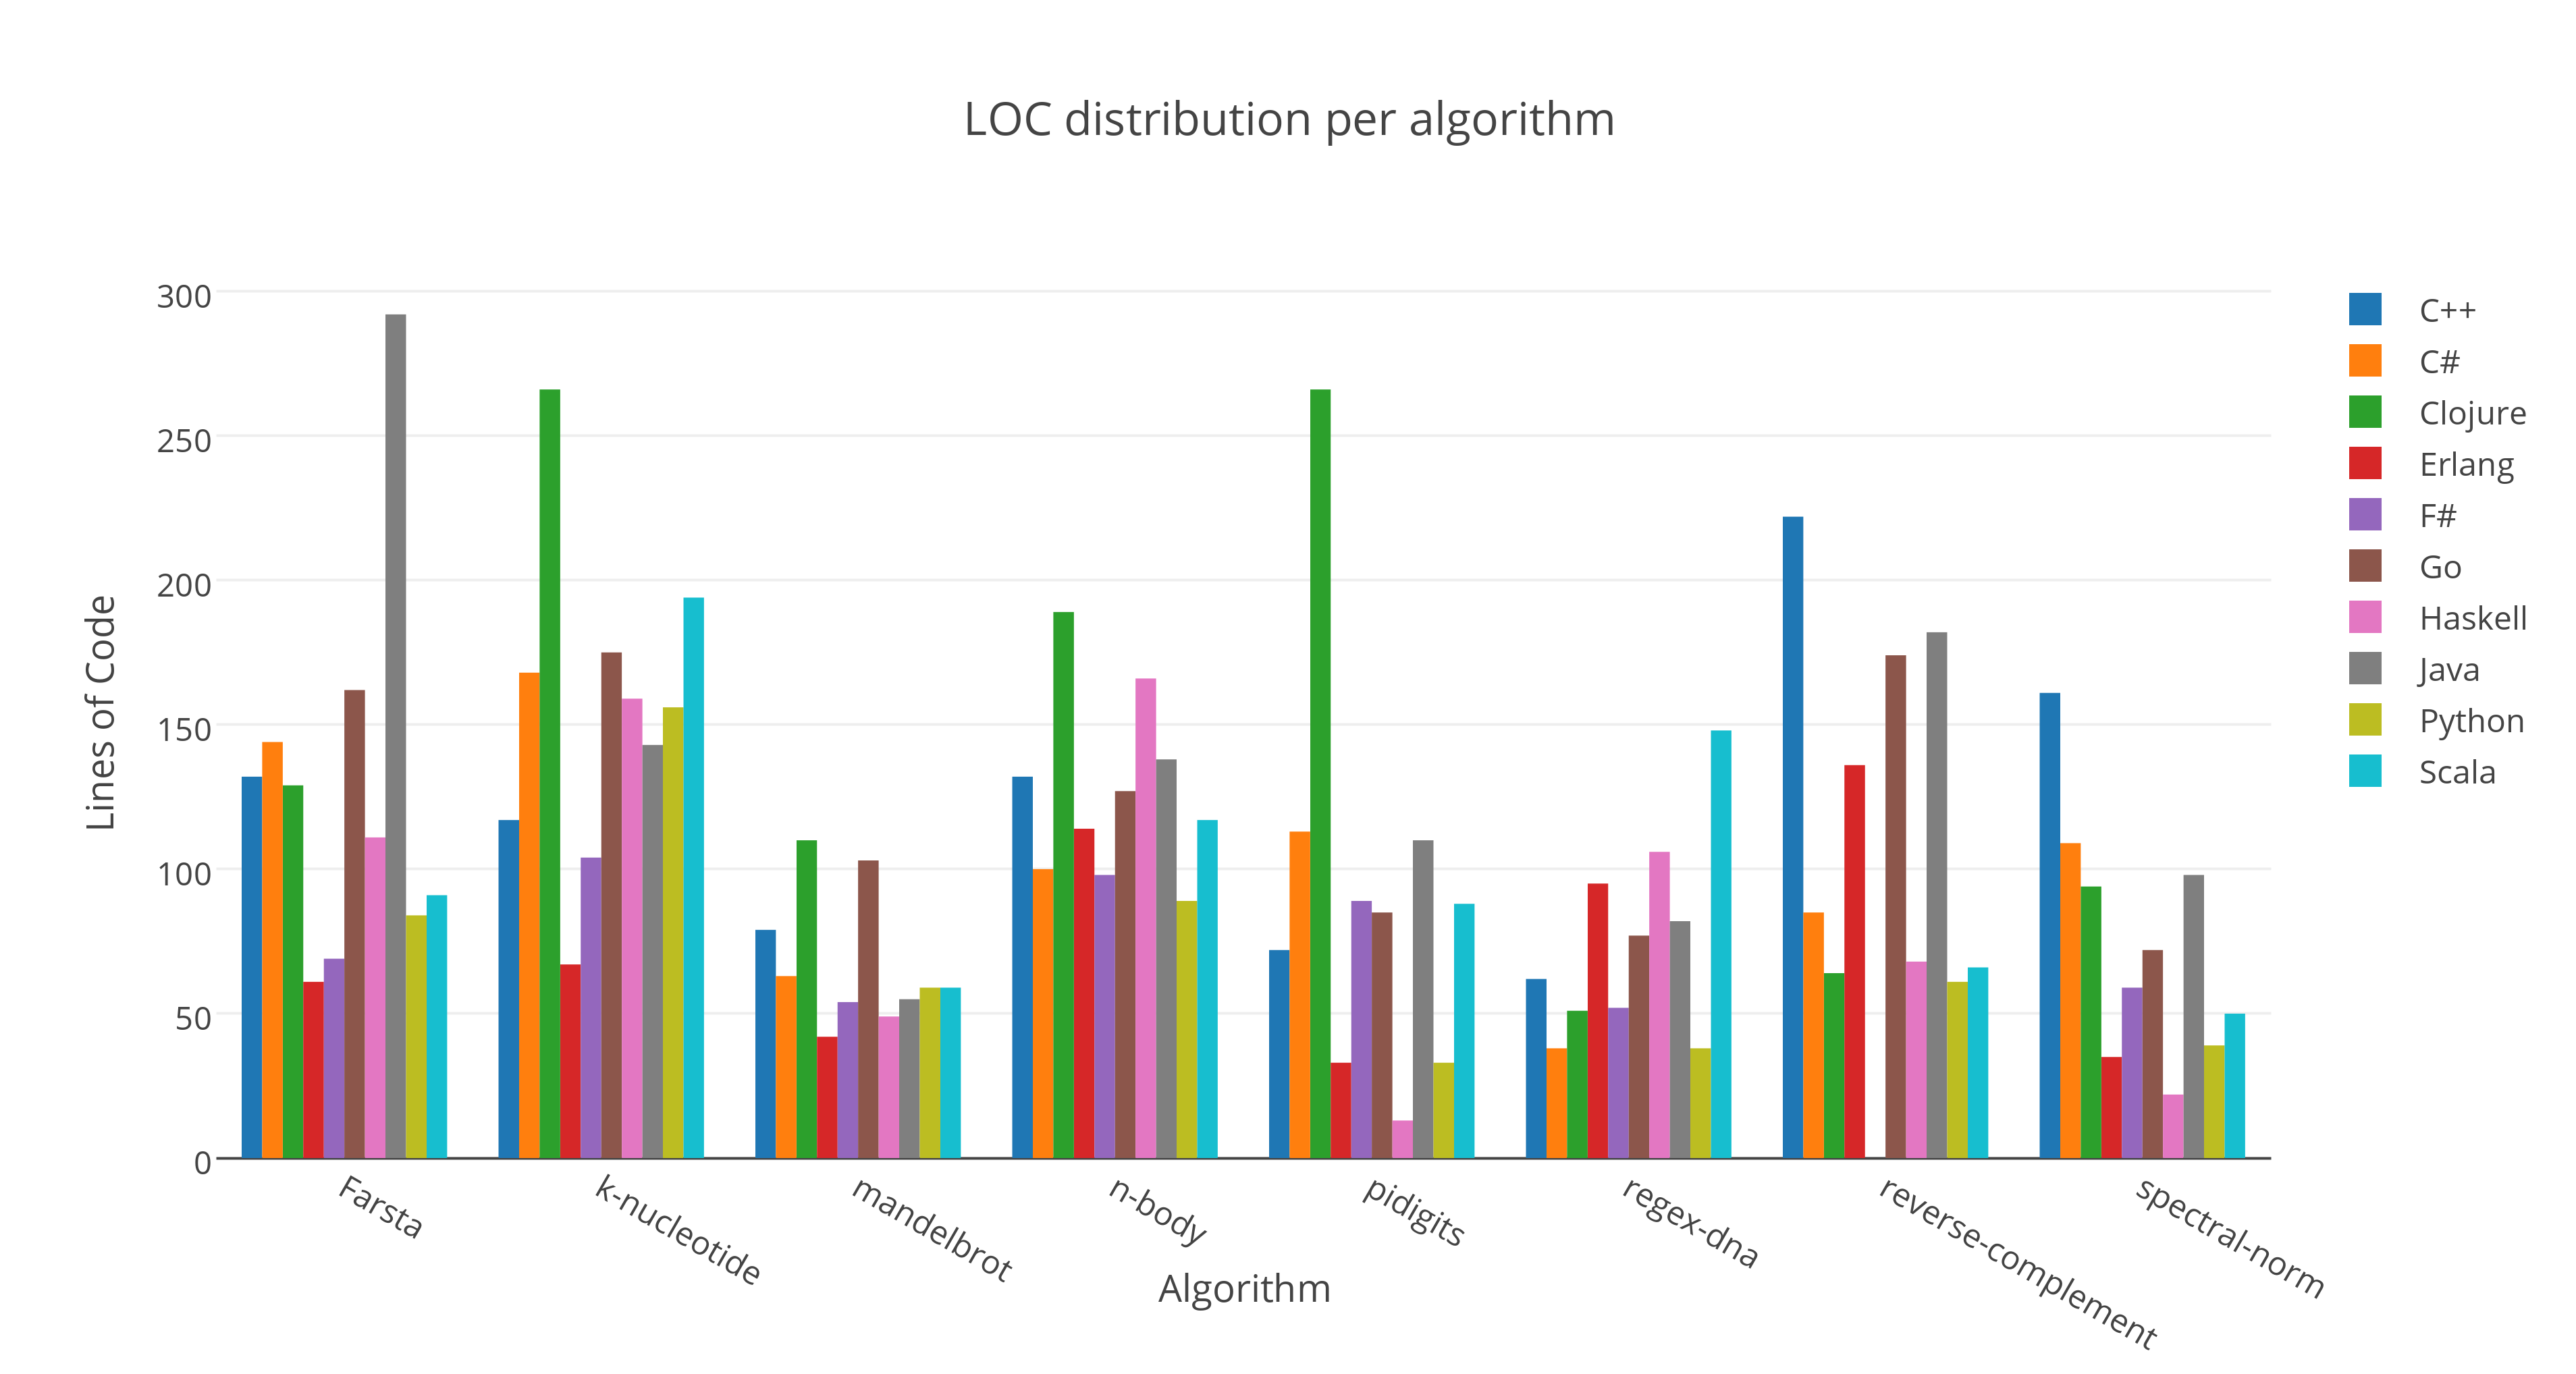
\includegraphics[width=\textwidth]{2}
\caption{The graph shows the distribution of the LOC of different languages implementation for different algorithms.}
\label{fig:alg}
\end{figure}

An alternative way to visualise these results is to think in terms of language and display which algorithms is the best to implement and be more productive. Fig \ref{fig:lang} shows this alternative representation.

\begin{figure}[h]
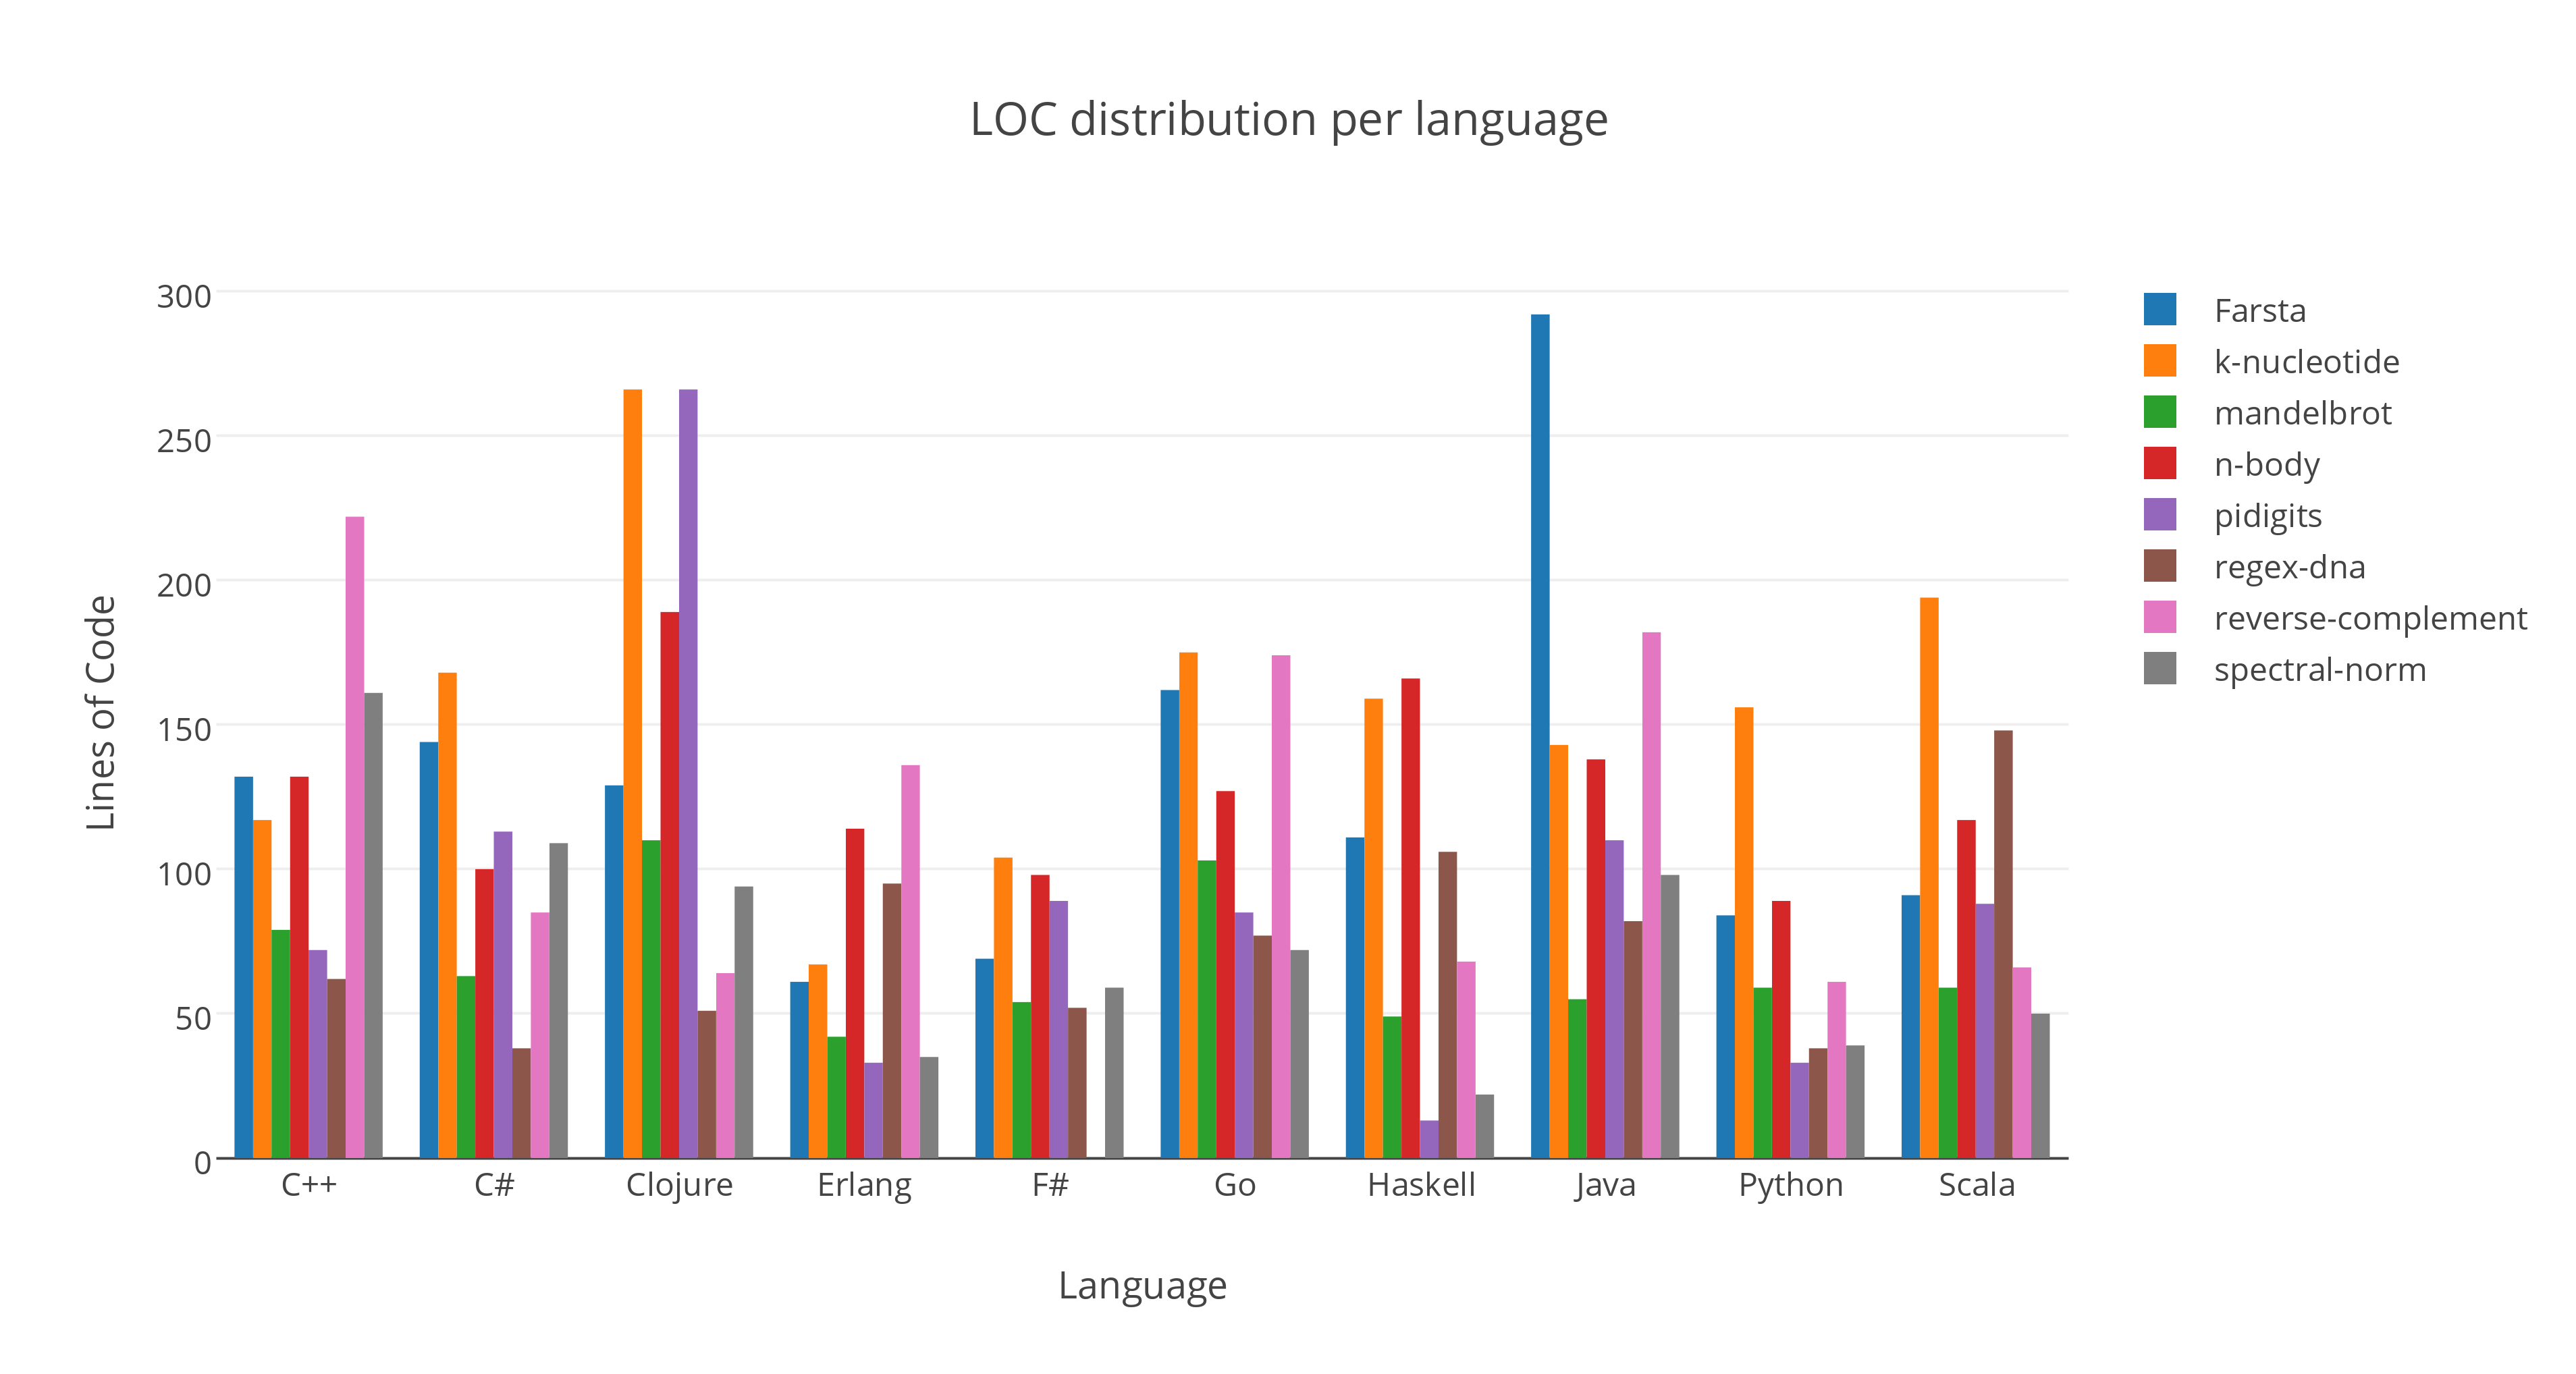
\includegraphics[width=\textwidth]{3}
\caption{The graph shows the LOC used to solve each algorithm for the same language.}
\label{fig:lang}
\end{figure}

The above graphs have the disadvantages to present too much information so that the readers may have trouble understanding which paradigm is more efficient. For this reason we synthesised the gathered data in a graph that shows only the average LOC for each paradigm per each algorithm. This representation of the data is shown in Fig. \ref{fig:fpvsoop}.

\begin{figure}[h]
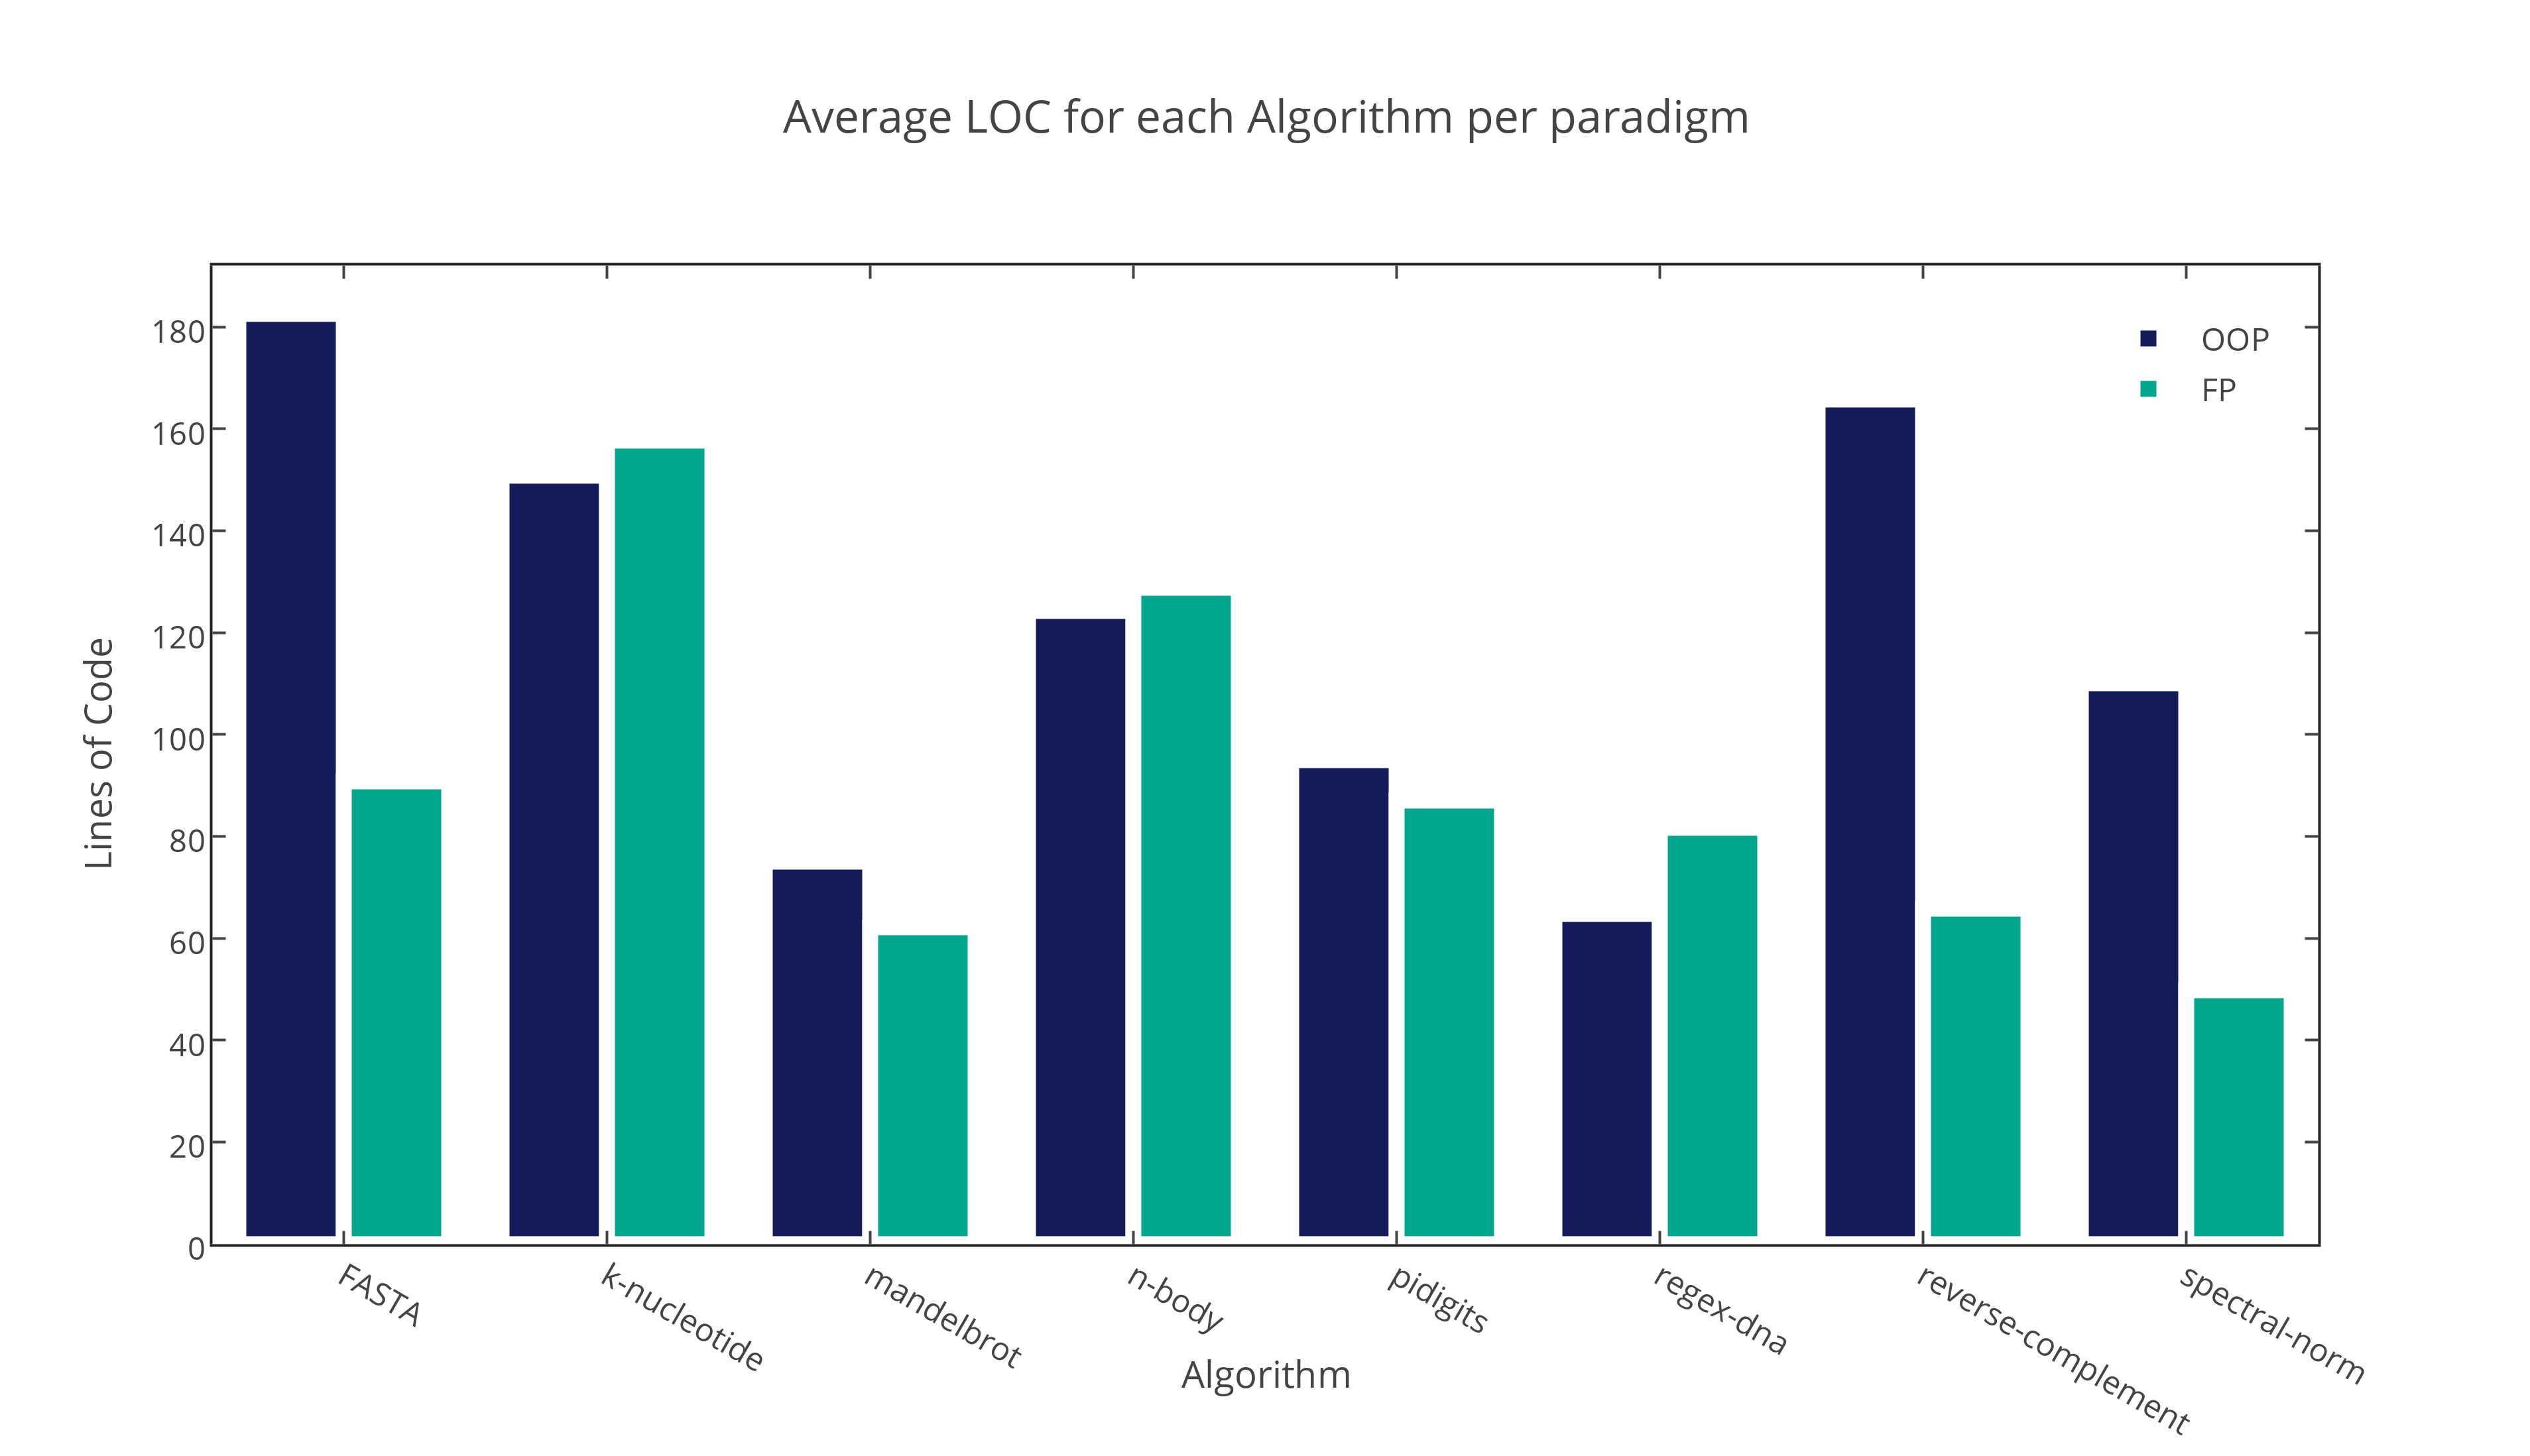
\includegraphics[width=\textwidth]{1}
\caption{The graph represents the distribution of both FP and OOP paradigm in different algorithms.}
\label{fig:fpvsoop}
\end{figure}

What we evince from the gathered data is that, normally, there is no big difference between the LOC for FP and OOP. Nevertheless, in certain algorithms the LOC in FP implementations are less than the half of OOP implementation.

\section{Discussion}

\section{Conclusion}

\bibliography{article}
\bibliographystyle{plain}

%\begin{thebibliography}{9}
%\bibitem{tiobe}
%http://www.tiobe.com/index.php/content/paperinfo/tpci/index.html
%\bibitem{flink}
%Apache Flink. 2015. Apache Flink: Scalable Batch and Stream Data Processing. [ONLINE] Available at: http://flink.apache.org. [Accessed 16 September 15].
%\bibitem{rx}
%ReactiveX. 2015. ReactiveX. [ONLINE] Available at: http://reactivex.io/. [Accessed 16 September 15].
%\bibitem{fpoop}
%R. Harrison, \enquote*{Comparing programming paradigms: an evaluation of functional and object-oriented programs}, Jul. 1996 [Online]. Available: http://ieeexplore.ieee.org/stamp/stamp.jsp?tp=\&arnumber=511273
%\bibitem{githubapi}
%GitHub Developer. 2015. Statistics | GitHub API. [ONLINE] Available at: https://developer.github.com/v3/repos/statistics/. [Accessed 16 September 15].
%\bibitem{benkio}
%https://github.com/benkio/ITC-Slides
%\end{thebibliography}

\end{document}